\documentclass[accepted]{tpm2023} % for initial submission
% \documentclass[accepted]{tpm2023} % after acceptance, for a revised
                  % version; also before submission to
                  % see how the non-anonymous paper
                  % would look like
%% There is a class option to choose the math font
% \documentclass[mathfont=ptmx]{tpm2023} % ptmx math instead of Computer
                     % Modern (has noticable issues)
% \documentclass[mathfont=newtx]{tpm2023} % newtx fonts (improves upon
                     % ptmx; less tested, no support)
% NOTE: Only keep *one* line above as appropriate, as it will be replaced
%    automatically for papers to be published. Do not make any other
%    change above this note for an accepted version.

%% Choose your variant of English; be consistent
\usepackage[american]{babel}
% \usepackage[british]{babel}

%% Some suggested packages, as needed:
\usepackage{natbib} % has a nice set of citation styles and commands
  \bibliographystyle{plainnat}
  \renewcommand{\bibsection}{\subsubsection*{References}}
\usepackage{mathtools} % amsmath with fixes and additions
\usepackage{amssymb,amsfonts,amsthm}
% \usepackage{siunitx} % for proper typesetting of numbers and units
\usepackage{booktabs} % commands to create good-looking tables
\usepackage{tikz} % nice language for creating drawings and diagrams
\usepackage{algorithm,algpseudocode}
\usepackage{xcolor}
\usepackage{tabularx}

%% Provided macros
% \smaller: Because the class footnote size is essentially LaTeX's \small,
%      redefining \footnotesize, we provide the original \footnotesize
%      using this macro.
%      (Use only sparingly, e.g., in drawings, as it is quite small.)

%% Self-defined macros
\newcommand{\TODO}[1]{\textbf{\color{red}{TODO: #1}}}
\DeclareMathOperator*{\ch}{ch}
\DeclareMathOperator*{\scope}{sc}

\algnewcommand{\LineComment}[1]{\State \(\triangleright\) #1}
\algnewcommand{\Input}[1]{\State \textbf{Input:} #1}
\algnewcommand{\Output}[1]{\State \textbf{Output:} #1}

\title{On Modal Clustering with Gaussian Sum-Product Networks}

% The standard author block has changed for TPM 2023 to provide
% more space for long author lists and allow for complex affiliations
%
% All author information is authomatically removed by the class for the
% anonymous submission version of your paper, so you can already add your
% information below.
%
% Add authors
\author[1]{\href{mailto:madeira@ime.usp.br}{Tiago Madeira}{}}
\author[1]{\href{mailto:ddm@ime.usp.br}{Denis Deratani Mauá}{}}
% Add affiliations after the authors
\affil[1]{%
 Institute of Mathematics and Statistics\\
 University of São Paulo\\
 Brazil
}

\begin{document}
\maketitle

\begin{abstract}
  Recent research highlights the significance of incorporating density modeling into clustering procedures.
  While the Sum-Product Networks' ability to compactly represent mixture models has been long noticed, their potential for modal clustering remains largely unexplored.
  This paper explores the use of Gaussian Sum-Product Networks for semi-parametric density-based clustering via mode association.
  To associate points to modes, we make use of a recently developed efficient EM-style algorithm.
  We perform image segmentation experiments to evaluate the (dis)advantages of modal clustering using such models.
\end{abstract}

\section{Introduction}
\label{sec:intro}

Clustering plays a pivotal role in data analysis, by which means one can discover segments of homogeneous examples (e.g., similar online purchases), detect outliers and anomalies, fill-in missing values, etc.
%Typically, one expects a cluster to be a relatively dense region of the sample space that is well separated from other dense regions \citep{clustering}.

Most clustering methods take a distance or dissimilarity function as input, and segment data so as to minimize intra-cluster distance and maximize inter-cluster distance \citep{clustering}.
The most prominent example is the $k$-means algorithm \citep{MacQueen1967}.
%
%The majority of clustering methods categorizes points in a dataset by mean of a distance function. Such methods proceed by selecting a partition of the dataset that optimizes a chosen objective function that favors small intra-cluster distance and large inter-cluster distance. For instance, the classical $k$-means algorithm repeatedly identifies $k$ cluster centers and assigns data points to the nearest cluster center, with the aim of minimizing the squared distances from the clusters \citep{MacQueen1967}.
%
More recently, an increasing number of researchers have emphasized the importance of more explicitly incorporating density modeling into clustering procedures \citep{Carlsson2013}.
%
%In this direction, \citet{Chacon2019} carried out a comparative study of two distinct density-based clustering approaches: mixture model clustering and modal clustering. 

Mixture models form an expressive class of density models, capable of approximating any well-behaved density.
A mixture model can be used for clustering either by associating each point to a component, or by associating each point to a mode.
The former approach should be favored when one has reason to believe that the true density aligns with the assumed latent-variable model \citep{Chacon2019}.
The latter is preferred when there is no particular reason to assume a specific parametric model of data.
Note that the modes and mixture components can differ significantly in number and location \citep{Amendola2019}.

%In situations where the true density aligns with the assumed class of mixture densities, mixture model clustering offers the capability to explore more intricate scenarios compared to modal clustering. 
%However, if mixture modeling is employed primarily to leverage the dense space of mixture densities as an approximation to any density, the association between clusters and mixture components becomes less reliable and raises questions.

Sum-Product Networks (SPNs) are a relatively recent class of deep statistical models that leverage arithmetic circuits \citep{Darwiche2003} to effectively capture context-sensitive independences and offer reliable and efficient inference, making them a competitive approach for a wide range of demanding machine learning tasks \citep{Poon2011, Llerena2017, Amer2016}.

While the connection of SPNs and (hierarchical) mixture models has long been noticed \citep{Peharz2014,Zhao2015}, the application of SPNs to clustering remains relatively unexplored.
This in spite of the fact that the widely-used schema for learning SPNs
employs hierarchical clustering to construct the network's structure \citep{Gens2013,Vergari2018}.

In this paper, we report the first results of our investigation about the effectiveness of modal clustering using Gaussian SPNs.
We discuss the advantages and difficulties with such an approach.
In particular, we discuss how to employ a recently developed EM-like algorithm for mode finding in Gaussian SPNs \citep{Madeira2022} to perform modal clustering, and show its application to image segmentation.
%, that extend previous work in modal clustering with mixture models \citep{Li2007}.
%We evaluate the techniques on an image segmentation task.


% We argue that SPNs, specifically those employing Gaussian distributions as inputs, have the ability to approximate any density and represent a Gaussian Mixture Model (GMM) with a substantially smaller number of components.
% As a result, they offer a promising approach for clustering based on the high-density regions within the GMMs they represent.

% In this paper, we investigate the effectiveness of clustering via mode identification using Gaussian SPNs.
% To find local maxima of a density, we use \emph{Modal EM} \citep{Li2007}, a method that is equivalent to a generalized \emph{Mean-Shift} \citep{Fukunaga1975} in the context of Gaussian mixtures.
% We conduct clustering experiments with image segmentation to visualize the effectiveness of our approach.

\section{Sum-Product Networks}
\label{sec:fundamentals}

A Sum-Product Network (SPN) is a weighted rooted directed acyclic graph, where each internal is either a sum node or a product node, and each leaf node corresponds is a univariate distribution \citep{Gens2013}.
The edges $u \rightarrow v$ from a sum node $u$ are associated with weights $w(u, v) \geq 0 $, and the remaining edges have weight 1 (usually omitted).
For any node $u$, we call its scope, denoted as $\scope(u)$, the set of random variables that appear in some distribution at the leaves of the inducing subgraph.

An SPN satisfies the properties of \emph{decomposability} and \emph{completeness}, which ensure that certain types of inferences are tractable.
Decomposability states that the scopes of any two children of a product node are disjoint (i.e., if $u$ is a product node then $\scope(v) \cup \scope(w) = \emptyset$ for any distinct $v,w \in ch(u)$).
Completeness states that the scopes of children of sum nodes are identical (i.e., if $u$ is a sum node then $\scope(v) = \scope(w)$ for any $v,w \in ch(u)$).
We also assume w.l.o.g.\ that the sum of the weights of edges from a sum node $u$ is 1, that is, $\sum_{v \in \ch(u)} w(u, v) = 1$.
Together, those three properties ensure that the SPN rooted at any node specifies a joint distribution over its scope.
This allow us to refer to nodes and their distribution functions interchangeably.


Given an SPN $\mathcal{S}$, we denote the value of its distribution at a configuration $\mathbf{x}$ of its scope $\mathbf{X}$ by $\mathcal{S}(\mathbf{x})$.
This value is obtained inductively as follows.
The value of a leaf node is the value of the corresponding distribution.
The value of an internal model is $\oplus_{v \in ch(u)} w(u,v) \mathcal{S}_v(\mathbf{x})$, where $\oplus$ is the operation of node $u$ (sum or product) and $\mathcal{S}_v$ is the SPN rooted at $v$.

%We denote its probability distribution function as $\mathcal{S}(\cdot)$. To compute the probability of a valuation $\mathbf{x}$ of RVs $\mathbf{X}$ in the SPN, $\mathcal{S}(\mathbf{X} = \mathbf{x})$, we traverse the graph in reverse topological order. For a node $u$, let $u(\mathbf{x})$ represent the value of node $u$ given the valuation $\mathbf{X} = \mathbf{x}$ restricted to the RVs in the scope of $u$. Then: (1) If $u$ is a leaf node, then $u(\mathbf{x})$ is the density of its corresponding univariate distribution; (2) If $u$ is a product node, $u(\mathbf{x})$ is the product of its children, i.e., $u(\mathbf{x}) = \prod_{v \in \ch(u)} v(\mathbf{x})$; (3) If $u$ is a sum node, $u(\mathbf{x})$ is the weighted sum of its children, i.e., $u(\mathbf{x}) = \sum_{v \in \ch(u)} w(u, v) v(\mathbf{x})$. The distribution of an SPN is the distribution of its root node.




% In this study, we impose two constraints on the SPNs under consideration: (1) For all sum nodes $u$, if a node $v$ belongs to the set of children $\ch(u)$, then $\scope(v) = \scope(u)$; (2) For all product nodes $u$, the scopes of its children are disjoint, i.e., if distinct nodes $v$ and $w$ are both in $\ch(u)$, then $\scope(v) \cup \scope(w) = \emptyset$. These constraints are commonly referred to as \emph{completeness} and \emph{decomposability} in the SPN literature, respectively.

% Every node in an SPN inherently represents a probability distribution over its scope. Specifically, leaves are distributions by definition, product nodes represent distributions under the assumption of independence among their children distributions, and sum nodes represent mixture distributions \citep{Peharz2015}.


Consider a subgraph $\mathcal{T}$ of an SPN $\mathcal{S}$. We say that $\mathcal{T}$ is an \emph{induced tree} if it can be constructed inductively, starting from the root of $\mathcal{S}$, and then including all children of product nodes and exactly one child of any sum node.
An induced tree $\mathcal{T}$ is a tree-shaped SPN (i.e., satisfies decomposability and completeness) whose distribution is given by
$\mathcal{T}(\mathbf{x}) = \prod_{u \rightarrow v \in \mathcal{T}} w(u, v) \prod_{j} T_j(\mathbf{x})$,
where $T_j$ is the SPN/distribution of the leaf of $\mathcal{T}$ whose scope is $X_j$ (note: $\mathcal{T}$ has exactly $n$ such leaves/variables).

Assume an ordering $\mathcal{T}^1,\dotsc,\mathcal{T}^{\tau}$ of the induced trees of $\mathcal{S}$, and let $w_i = \prod_{u \rightarrow v \in \mathcal{T}^i} w(u,v)$ be the product of the weights in the $i$-th induced tree.
Then, $\mathcal{S}(\mathbf{x}) = \sum_{i=1}^{\tau} w_i T^i(\mathbf{x})$ for any configuration $\mathbf{x}$ of the scope, where $T^i(\mathbf{x}) = \prod_{j=1}^n T_j^i(\mathbf{x})$ is the product of the values of the univariate distributions at the leaves for $X_j = x_j$.
Thus, induced trees provide an interesting representation of SPNs as a finite mixture model \citep{Zhao2016}, one where each induced tree represents a different component.
%Note that unlike trypical mixture models, an SPN has quite some level of redundancy or parameter-sharing among different components, given by the weights and univariate distributions they share.

In this study, our emphasis lies on SPNs with Gaussian distributions assigned to their leaves, known as Gaussian SPNs (or GSPNs, for short).
For such models, the resulting induced tree representation corresponds to a Gaussian Mixture Model (GMM), one where the variables in each component $\mathcal{T}^i$ are uncorrelated and have mean $\sigma_{k_i}$ and variance $\sigma_{k_i}^2$.

\section{Modal clustering in GSPNs}
\label{sec:mem}

In modal clustering, data points are segmented by associating each point to a mode of a density model, usually by means of some hill-climbing strategy.
Hence, to employ Gaussian SPNs for such intent one needs a method that identifies (some of) its modes.

\subsection{Finding modes}

\citet{Li2007} developed the \emph{Modal EM}, an EM-style method that finds a mode of a GMM $p(\mathbf{x}) = \sum_k^\tau w_k p^k(\mathbf{x})$ by hill-climbing from a given starting point $\mathbf{x}^{(0)}$.
The method alternates the following two steps until convergence:

\begin{description}
  \item[E-step:] Let
    $q_k = \frac{w_k p^k\left(\mathbf{x}^{(r)}\right)}{p\left(\mathbf{x}^{(r)}\right)},
      \text{ for } k = 1, \cdots, \tau \, .$

  \item[M-step:] Compute
    $\mathbf{x}^{(r+1)} = \arg\max_\mathbf{x} \sum_k^\tau q_k \log p^k\left(\mathbf{x}\right) \, .$
\end{description}

The direct application of the above algorithm to SPNs is intractable due to the high number of components (given by its number of induced trees).
To overcome that limitation, \citet{Madeira2022} adapted Modal EM to exploit the recursive character of GSPNs.
Their algorithm repeatedly obtains a configuration $\mathbf{x}^{(r+1)}$ from a configuration $\mathbf{x}^{(r)}$ by:
\begin{equation}
  \label{eq:memspns}
  x^{(r+1)}_i = \frac{\sum_k^\tau \frac{\mu_{k_i}}{\sigma_{k_i}^2} w_k T^k\left(\mathbf{x}^{(r)}\right)}{\sum_k^\tau \frac{1}{\sigma_{k_i}^2} w_k T^k\left(\mathbf{x}^{(r)}\right)} \, .
\end{equation}
The equation above is computed by traversing the network from the leaves to the root, taking time $\Theta(n|\mathcal{S}|)$ per iteration, where $n$ is the number of random variables and $|\mathcal{S}|$ is the number of nodes in the SPN.


%\noindent The algorithm traverses the network from bottom to top, and each node propagates $2n$ values, which correspond to the numerator and denominator of Equation \ref{eq:memspns} for each $X_i$.
% Its pseudo-code is presented in Algorithm \ref{alg:mem}.

% \begin{algorithm}
% \centering
% \caption{Modal EM for GSPNs}
% \label{alg:mem}
% \begin{algorithmic}
% \Input{a GSPN $\mathcal{S}$ over $X_1, \cdots, X_d$, and $\mathbf{x}^{(r)} \in \mathbb{R}^d$}
% \Output{a point $\mathbf{x}^{(r+1)} \in \mathbb{R}^d$ s.t. $\mathcal{S}\left(\mathbf{x}^{(r+1)}\right) \geq \mathcal{S}\left(\mathbf{x}^{(r)}\right)$}
% \end{algorithmic}
% \begin{algorithmic}[1]
% \ForAll{node $u$ of $\mathcal{S}$ in reverse topological order}
% \If{$u$ is a leaf}
% \LineComment{Let $X_i$ be the RV in the scope of $u$;}
% \LineComment{Let $\mu$ and $\sigma$ be the parameters of $u$.}
% \State $N^u_i \gets \frac{u\left(x^{(r)}_i\right)\mu}{\sigma^2}$, $D^u_i \gets \frac{u\left(x^{(r)}_i\right)}{\sigma^2}$ \label{alg:mem:leaf:1}
% \ForAll{RV $X_j \neq X_i$}
% \State $N^u_j \gets D^u_j \gets u\left(x^{(r)}_i\right)$ \label{alg:mem:leaf:2}
% \EndFor
% \ElsIf{$u$ is a product node}
% \ForAll{RV $X_i$} \label{alg:mem:product}
% \State $N^u_i \gets \prod_{v \in \ch(u)} N^v_i$
% \State $D^u_i \gets \prod_{v \in \ch(u)} D^v_i$
% \EndFor
% \ElsIf{$u$ is a sum node}
% \ForAll{RV $X_i$} \label{alg:mem:sum}
% \State $N^u_i \gets \sum_{v \in \ch(u)} w(u, v) N^c_i$
% \State $D^u_i \gets \sum_{v \in \ch(u)} w(u, v) D^v_i$
% \EndFor
% \EndIf
% \EndFor
% \State \Return{$\frac{\mathbf{N}^\text{root}}{\mathbf{D}^\text{root}}$} \label{alg:mem:return}
% \end{algorithmic}
% \end{algorithm}

Notably, the updates in Equation \ref{eq:memspns} coincide with the fixed-point iterative scheme proposed by \citet{Carreira-Perpinan2000} for finding modes of GMMs.
In turn, this iterative scheme can be seen as a generalized version of the famous Mean-Shift algorithm \cite{Chacon2019}.

%\TODO{Discuss convergence.}

\subsection{On the number of clusters}

In modal clustering, the number of clusters corresponds to the number of modes in the model (and not to the number of components).
A precise characterization of the relation of number of modes $m(d, k)$ as a function of the number of components $k$ and dimensionality $d$ is still an open problem.
\citet{Amendola2019} showed that $m(d, k) \geq {k \choose d} + k$ for $d, k \geq 2$,.
Additionally, they established that the number of non-degenerate stationary points of a $d$-dimensional GMM with $k$ components is bounded above by $2^{d+{k \choose 2}}(5+3d)^k$.
These bounds suggest that the number of modes can vary greatly inside a class of mixture models of same complexity.

We note that in SPNs the number of components ($k$) is not usually specified and is rather induced from data.

%% TODO: Add figure showing example of density with more/less modes than components and cite here.

%While density models with an exponentially larger number of modes in the number of components can be easily constructed, folk knowledge assumes that GMMs learned from data typically have many more components than nodes.

%Therefore, understanding the maximum number of modes a $d$-dimensional Gaussian mixture with $k$ components can have is of interest. Let $m(d, k)$ represent this maximal number of modes.

%Previous research by \citet{Amendola2019} has provided the most stringent lower and upper bounds for $m(d, k)$ to date. For $d, k \geq 2$, they have shown that a mixture of $k$ Gaussians in $d$ dimensions can have at least ${k \choose d} + k$ modes, i.e., $m(d, k) \geq {k \choose d} + k$. Additionally, they established that the number of non-degenerate stationary points for a $d$-dimensional GMM with $k$ components is bounded by $2^{d+{k \choose 2}}(5+3d)^k$. These bounds provide insights into the potential number of modes in Gaussian mixture models.

%The number of clusters discovered in modal clustering with SPNs is highly influenced by the choice of learning algorithm and its corresponding hyperparameters.

\section{Image Segmentation}
\label{sec:experiments}

As a preliminary investigation of the effectiveness of modal clustering with GPSNs, we performed some experiments with image segmentation of two images, shown in Figure \ref{fig:originals}.

\begin{figure}
  \centering
  \begin{minipage}{0.2\textwidth}
    \centering
    \scalebox{0.15}{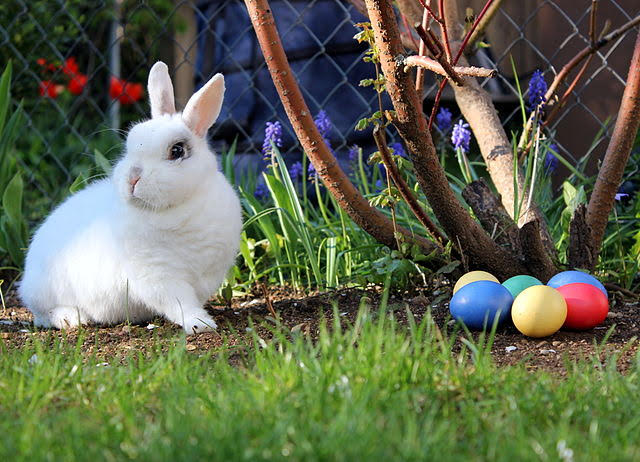
\includegraphics{rabbit.jpg}}

    (a)
  \end{minipage}\begin{minipage}{0.2\textwidth}
    \centering
    \scalebox{0.087}{
\includegraphics{tarsila3.jpg}}

    (b)
  \end{minipage}

  \caption{(a) Easter Bunny. (b) Tarsila do Amaral's The Family.}
  \label{fig:originals}
\end{figure}

We obtained datasets of 5 variables by considering the RGB intensity values and $x$ and $y$ locations of each pixel in the image.
%Each instance in the dataset includes the pixel's $x$ and $y$ coordinates, along with three color values representing the pixel's red, green, and blue components on a scale of 0 to 255. 
This resulted in $200 \times 144 = 28,800$ data points (instances) for Easter Bunny and $200 \times 158 = 31,600$ for The Family.
%
The datasets were then used to learn GSPNs from data, using the LearnSPN implementation provided by the SPFlow library.\footnote{Available at \url{github.com/SPFlow/SPFlow}.} Instance splitting was performed using GMM clustering, while variable splitting was accomplished using the Randomized Dependence Coefficient \citep{Lopes-Paz2013}.
We compared our implementation of Modal EM clustering with $k$-means clustering, as implemented by the scikit-learn library.\footnote{Available at \url{scikit-learn.org}.}

We experimented with different GSPNs by varying the minimum number of instances required for slicing in the learning process ($s$).
Tables \ref{tab:segmentation-rabbit} and~ \ref{tab:segmentation-tarsila} show the number of nodes, network height and the number of clusters (modes) obtained for each GSPN as we vary $s$.
One sees the great dependence between those quantities, as well as the quick increase in the number of modes.

\begin{table}
  \centering
  \caption{SPNs Learned for Segmentation (Easter Bunny).}
  \label{tab:segmentation-rabbit}

  \begin{tabular}{rrrr}
    \toprule
    \bfseries Parameter $s$ & \bfseries Nodes & \bfseries Height & \bfseries Clusters \\ \midrule
    20,000                  & 13              & 3                & 6                  \\
    15,000                  & 19              & 3                & 7                  \\
    10,000                  & 25              & 3                & 10                 \\
    5,000                   & 50              & 5                & 31                 \\
    2,000                   & 132             & 5                & 68                 \\
    500                     & 528             & 7                & 398                \\
    200                     & 1,267           & 9                & 676                \\
    \bottomrule
  \end{tabular}
\end{table}

\begin{table}
  \centering
  \caption{SPNs Learned for Segmentation (The Family).}
  \label{tab:segmentation-tarsila}

  \begin{tabular}{rrrr}
    \toprule
    \bfseries Parameter $s$ & \bfseries Nodes & \bfseries Height & \bfseries Clusters \\ \midrule
    20,000                  & 13              & 3                & 4                  \\
    15,000                  & 25              & 3                & 5                  \\
    10,000                  & 31              & 3                & 8                  \\
    5,000                   & 61              & 3                & 19                 \\
    2,000                   & 163             & 3                & 43                 \\
    500                     & 603             & 7                & 187                \\
    200                     & 1,504           & 7                & 555                \\
    \bottomrule
  \end{tabular}
\end{table}

\newcommand{\segfigrow}[3]{
  \begin{minipage}{0.1\textwidth}
    \centering
    $s = #2$\\$k = #3$
  \end{minipage}    &
  \begin{minipage}{0.12\textwidth}
    \centering
    \scalebox{0.29}{\includegraphics{fixed_mem_recolored_#1_200_#2_0.300000.png}}
  \end{minipage} &
  \begin{minipage}{0.12\textwidth}
    \centering
    \scalebox{0.29}{\includegraphics{k_#3_recolored_#1_200.png}}
  \end{minipage}
}

%The image was segmented by coloring each pixel according to the mode to which Modal EM converged when initialized with the corresponding values (taking the color of the mode).
The images were segmented by coloring each pixel according to the average color of the pixels in its same cluster, considering a cluster to be formed by points which converge to the same mode.
Figures \ref{fig:bunny} and~\ref{fig:tarsila} display a visual comparison of image segmentation by GSPNs and by the $k$-means algorithm, where $k$ is set to the number of clusters identified by Modal EM in GSPNs trained with different hyperparameters.
% Each pixel is recolored using the color of its cluster center.
One can note that GSPN seemingly delivers a worse segmentation than $k$-means, while taking much more compute.
We conjecture that GSPN's worse performance is due to a lack of fit to the model, which could be mitigated by changing the structure learning algorithm, performing fine-tuning of parameters or even using $k$-means solution as a initial model for refinements.

\begin{figure}
  \centering
  \begin{tabular}{ccc}
    %\toprule
    %\bfseries Parameters
     & \bfseries GSPN & \bfseries $k$-means \\ %\midrule
    \segfigrow{rabbit}{20000}{6}            \\ %\\
    \segfigrow{rabbit}{10000}{10}           \\ %\\
    \segfigrow{rabbit}{2000}{68}            \\ %\\
    \segfigrow{rabbit}{500}{398}                                %\\
    %\bottomrule
  \end{tabular}
  \caption{Image Segmentation of Easter Bunny.}
  \label{fig:bunny}
\end{figure}

\begin{figure}
  \centering

  \begin{tabular}{ccc}
    %\toprule
    %\bfseries Parameters
     & \bfseries GSPN & \bfseries $k$-means \\ %\midrule
    \segfigrow{tarsila3}{20000}{4}          \\ %\\
    \segfigrow{tarsila3}{10000}{8}          \\ %\\
    \segfigrow{tarsila3}{5000}{19}          \\ %\\
    \segfigrow{tarsila3}{500}{187}                              %\\
    %\bottomrule
  \end{tabular}
  \caption{Image Segmentation of The Family.}
  \label{fig:tarsila}
\end{figure}

To conclude, we note that GSPN modal clustering can deliver inferences that standard clustering techniques such as $k$-means cannot, such as coping with missing values, detecting outliers by probability threshold and scaling up easily to more complex and high-dimensional domains.

\section{Conclusions}
\label{sec:conclusions}

In this paper, we have presented an initial exploration of modal clustering using SPNs. Our experiments have highlighted the significant influence of the hyperparameters used to learn the SPN on the resulting number of modes in the model, underscoring the crucial role of parameter selection in achieving desired clustering outcomes.

Furthermore, our findings have demonstrated the applicability of clustering techniques for SPN model analysis. The number of modes in a density distribution serves as an indicator of the complexity of the underlying model, providing valuable insights into its representation capabilities.

While image segmentation may not be the optimal application domain for SPNs, our results have shown satisfactory performance comparable to the widely-used $k$-means algorithm. However, visually, we observed that image segmentation using $k$-means with $k$ equivalent to the number of modes in the SPN yields more detailed segmentation results.

We acknowledge that there is ample room for future work, particularly in exploring the application of modal clustering in various domains beyond image segmentation. These directions can contribute to expanding the understanding and utility of SPNs in clustering tasks across diverse fields.

\begin{acknowledgements}

  This work was partially financed by CNPq grant \#305136/2022-4, CAPES Finance Code 001 and FAPESP grant \#2022/02937-9.
\end{acknowledgements}
\bibliography{references}
\end{document}
